
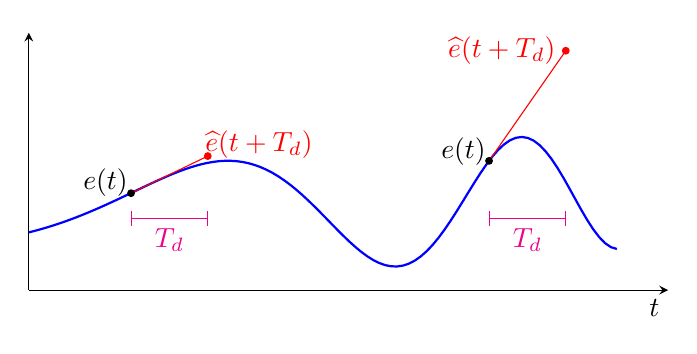
\begin{tikzpicture}
\pgfplotsset{width=0.8\columnwidth,height=0.4\columnwidth}


\begin{axis}[
       ymin=0,
       ymax=2.15,
       xmax=27,
       xlabel={$t$},
       every axis x label/.style=
         {at={(current axis.right of origin)},
          anchor=north,xshift=-5},
       axis x line = bottom,axis y line = left,
       ticks=none,
       clip=false,
]

\addplot[blue,thick,domain=2:25, samples=100]
        {0.5+sin(x-5)+0.5*sin(x^2))};

\addplot[black,only marks, mark=*, mark size=1.2pt]
     coordinates{(6,0.81)};
\node[black] at (axis cs:5,0.9) {$e(t)$};
\draw[red]
     (axis cs:6,0.81) -- (axis cs:9,1.12);
\draw[|-|,magenta]
     (axis cs:6,0.6) --
     node[pos=0.5,below]{$T_d$}
     (axis cs:9,0.6);
\addplot[red,only marks, mark=*, mark size=1.2pt]
     coordinates{(9,1.12)};
\node[red] at (axis cs:11,1.22)
     {$\widehat{e}(t+T_d)$};

\addplot[black,only marks, mark=*, mark size=1.2pt]
        coordinates{(20,1.08)};
\node[black] at (axis cs:19,1.16) {$e(t)$};
\draw[red]
     (axis cs:20,1.08) -- (axis cs:23,2);
\draw[|-|,magenta]
     (axis cs:20,0.6) --
     node[pos=0.5,below]{$T_d$}
     (axis cs:23,0.6);
\addplot[red,only marks, mark=*, mark size=1.2pt]
     coordinates{(23,2)};
\node[red] at (axis cs:20.5,2)
     {$\widehat{e}(t+T_d)$};

\end{axis}


\end{tikzpicture}
